\documentclass[smaller,dvipsnames,ratio=169]{beamer}

\usetheme[numbering=fraction,%
          block=fill,%
          sectionpage=progressbar,%
          subsectionpage=progressbar,%
  ]{metropolis} % Use metropolis theme
\setbeamercovered{invisible}
\usepackage{graphicx}
\graphicspath{ {.} }

%\usepackage[round]{natbib} 
%\bibliographystyle{plainnat}
%\usepackage{natbib}
%\bibliography{literature.bib}

\usepackage[utf8]{inputenc}
\usepackage{xcolor}
\usepackage{xspace}
\usepackage{comment}
\usepackage{booktabs}
\usepackage{amssymb}
\usepackage{smartdiagram}
\usepackage{tikz}
  \usetikzlibrary{arrows} % required in the preamble
\usepackage{listings}
\usepackage{todonotes}

\title{On Commonsense Domains within\\ the Winograd Schema Challenge
}
\subtitle{Research Project}
\author[author1]{Aneta~Koleva\\[10mm]{\small Supervisors: Prof. Sebastian Rudolph \hspace{10mm} Dr. Emmanuelle Dietz}}

\institute{Dresden University of Technology\\[2mm] } 
\date{28-03-2019}

\begin{document}

  \maketitle

  %\section{Introduction}

  \begin{frame}{Motivation}
  	
	\onslide<1->\begin{itemize} 	
		\item Winograd Schema Challenge (Levesque et. al, 2012)
			\begin{itemize}
				\normalsize
				\item[S:] The trophy does not fit into the brown suitcase\\ because \alert{it} is too \alert{[small/large]}.
				\item[Q:] What is too [small/large]?
				\item[A:] The suitcase/the trophy.
			\end{itemize}	
		
	\end{itemize}
\onslide<2->		\centering
					%\documentclass{article}
%\usepackage{tikz}
%\begin{document}
\begin{comment}
	content...

	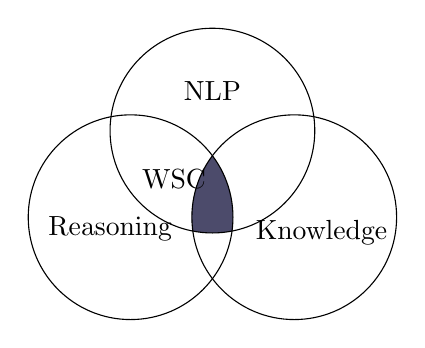
\begin{tikzpicture}
	\definecolor{Psy}{HTML}{4C4B6B}
	 \begin{scope}%[blend group=soft light]
	 
	 \def\firstcircle{( 90:0.5) circle (1.3cm)}
	 \def\secondcircle{(210:1.2) circle (1.3cm)}
	 \def\thirdcircle{(330:1.2) circle (1.3cm)}
	    \fill[white]  \firstcircle;
		 \fill[white] \secondcircle;
		 \fill[white] \thirdcircle;
		 
			 
		  \begin{scope}
		\clip \firstcircle;
		\clip \secondcircle;
		\fill[Psy] \thirdcircle;
		\end{scope}
			 
		 \draw \firstcircle;
		 \draw \secondcircle;
		 \draw \thirdcircle;
		 
		 \node at ( 90:1)    {NLP};
		 \node at (210:1.5)    {Reasoning};
		 \node at (330:1.6)    {Knowledge};
		 \node at (193:0.5) {WSC};
	\end{scope}	 
	\end{tikzpicture}
%
\end{comment}

\begin{figure}[width]
	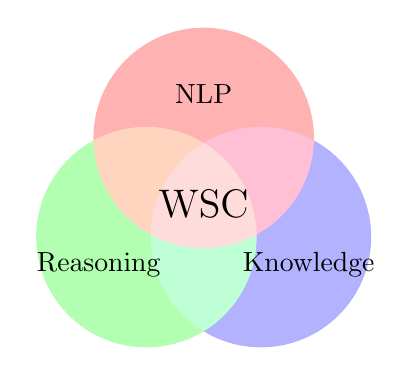
\begin{tikzpicture}[scale = 0.7]
	\begin{scope}[blend group = soft light]
	\fill[red!30!white]   ( 90:1.2) circle (2);
	\fill[green!30!white] (210:1.2) circle (2);
	\fill[blue!30!white]  (330:1.2) circle (2);
	\end{scope}
	\node at ( 90:2)    {NLP};
	\node at ( 210:2.2)   {Reasoning};
	\node at ( 330:2.2)   {{Knowledge}};
	\node [font=\Large] {WSC};
	\end{tikzpicture}
\end{figure}

%\end{document}%
\end{frame}

\begin{frame}{Outline}
	\tableofcontents
\end{frame}

\section{Description}

\begin{frame}{Winograd Schema Challenge} 
		%\footnote{Levesque et. al, The Winograd Schema Challenge, 2012}}
\onslide<1->	\begin{itemize}
		\small
		\item[S:] The trophy does not fit into the brown suitcase\\ because \alert{it} is too \alert{[small/large]}.
		\item[Q:] What is too [small/large]?
		\item[A:] The suitcase/the trophy
	\end{itemize} 
\onslide<2->\begin{itemize}
	\item Winograd Schema: 
	\begin{itemize}
		\normalsize
		\item Sentence containing two nouns, \\one ambiguous \alert{pronoun} and a special word
		\item Question asking about the referent of the pronoun
		\item Two possible answers corresponding to\\ the noun phrases in the sentence
	\end{itemize}
\onslide<3->	 \item Characteristics:
\onslide<3->	  \begin{itemize}
	  	\normalsize
	  	\item Easy to answer for an adult English speaker
	  	\item Always contains \alert{special word}
	  	\item Google proof
	  \end{itemize}
\end{itemize}
\end{frame}

\begin{frame}{Competition}
	
	\begin{itemize}
		\normalsize
		\item Competition in 2016 at IJCAI-16
		\begin{itemize}
			\normalsize
			\item Two time-constraint rounds - 210 min. each
		\begin{itemize}
			\normalsize
			\item Pronoun Disambiguation Problems (PDPs) - 60
			\item Parts of Winograd Schemas - 150
		\end{itemize}
		\item Four competitors
		\item Best result: 58\% correctly resolved PDPs
		\item There was no second round
		
		\end{itemize}
	
	\item Current \alert{state-of-the-art} (Radford et. al, 2019) achieves 70.7\% accuracy\\ on the WSs dataset
	\end{itemize}
	
\end{frame}


\begin{comment}
\begin{itemize}
\item [Text:] When they had eventually calmed down a bit, and had gotten home, Mr. Farley put the magic pebble in an iron safe. Some day they might want to use it, but really for now, what more could they wish for?

\item [Snippet:] to use it
\item [Answers:] magic pebble/safe

\end{itemize}

\end{comment}
\section{Previous Approaches}

\begin{frame}{Previous Approaches}
	\begin{itemize}
		\item Machine learning and deep learning
		\begin{itemize}
			\normalsize
			\item Supervised ranking SVM 
			\item Supervised classification Task 
			\item Knowledge enhanced embeddings 
			\item Google's language models 
			\item Open AI language model 
		\end{itemize}			
		\item Knowledge-based
		\begin{itemize}
			\normalsize
			\item Knowledge graphs with Relevance Theory 
			\item Semantic parsing and knowledge hunting 
			\item Parsing query results and assigning scores 
			\item Knowledge types identification 
		\end{itemize}
	\end{itemize}
\end{frame}

\begin{frame}{A Simple Method for Commonsense Reasoning\\ (Trinh and Le, 2018)}
	\begin{itemize}
		\normalsize
\onslide<1->		\item \alert{Language models} trained on unlabeled data
\onslide<2->		\begin{itemize}
			\normalsize
			\item Recurrent Neural Networks
			\item Trained on large datasets and on a dataset \alert{customized} for WSC
		\end{itemize}
\onslide<3->		\item Substitution ambiguous pronoun
\onslide<3->		\begin{itemize}
			\normalsize
			\item The trophy doesn't fit in the suitcase because\\ the \alert{trophy} is too big
			\item The trophy doesn't fit in the suitcase because\\ the \alert{suitcase} is too big
    	\end{itemize}
\onslide<4->		\item Language models assign probabilities to both sentences

\onslide<5->	\item Evaluation and results
		\begin{itemize}
			\normalsize
			\item PDPs 70\% accuracy
			\item WSC \alert{63.7\%} accuracy
		\end{itemize}
	\end{itemize}
\end{frame}

\begin{frame}{Knowledge Types Identification and Reasoning \\(Anonymous Authors,2019)}
	
\onslide<1->	\begin{itemize}
		\normalsize
		\item Identified 12 \alert{knowledge types} which cover the entire WSC dataset
		\item Developed a \alert{logical reasoning algorithm} 
		\item Evaluated on 100 problems from WSC and achieved \alert{100\%} accuracy
\onslide<2->		\item Solver
\onslide<2->		\begin{enumerate}
			\normalsize
			\item Semantic graph\footnote{kparser.org} of the input sentence and question
			\item Semantic graph representation of background knowledge
			\item Graph merging
			\item Project question graph on the merged graph
			\item Answer - the node from the merged graph which is from the same domain as the unknown node from the question graph
		\end{enumerate}
	\end{itemize}
		%\input{Figure4.png}
\end{frame}

\begin{frame}
	\begin{itemize}
		\normalsize
		\item Representation of the knowledge ``\textit{weak y \textbf{prevents} y lifts}"
	\end{itemize}
	
		\centering
		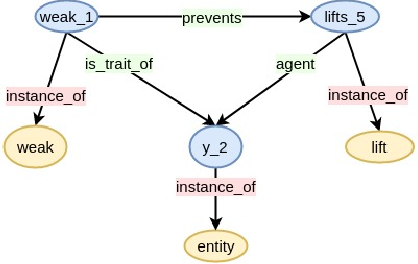
\includegraphics[scale=0.3]{Figure4_c.png}  
	
   
\end{frame}

\section{Methodology}

 \begin{frame}{Categorization of Winograd Schemas}
\onslide<1->	\begin{itemize}		
		\normalsize
		\item Motivation
		\begin{itemize}
			\normalsize
			\item Current state-of-the-art has a poor performance
			\item Background knowledge is crucial for predicting\\ the correct answer 
\onslide<2->			\item Idea
\onslide<2->		\begin{enumerate}
			\normalsize 
			\item Analyze the input Winograd Schema \\and identify the domain
			\item Search for knowledge \alert{specific} to this domain
			\item Apply reasoning procedure 
		\end{enumerate}
		\end{itemize}
	\end{itemize}   
\end{frame}

  \begin{frame}{Identified Categories}
  	\resizebox{\textwidth}{!}{

	\begin{tabular}{  l | l  }
		\hline
		\textbf{Category}  & \textbf{Example} \\ \hline
		1. Physical &\textbf{S:} John couldn't see the stage with Billy in front of him because he is so \textbf{[short/tall]}.\\&\textbf{Q:} Who is so [short/tall]? \\\hline
		
		2. Emotions &\textbf{S:}  Frank felt \textbf{[vindicated/crushed]} when his longtime rival Bill\\&revealed that he was the winner of the competition.\\&\textbf{Q:} Who was the winner of the competition?\\\hline
		
		3. Interactions &\textbf{S:} Joan made sure to thank Susan for all the help she had \textbf{[given/received]}. \\&\textbf{Q:} Who had [given/received] help?\\ \hline
		
		4. Comparison &\textbf{S:} Joe's uncle can still beat him at tennis, even though he is 30 years \textbf{[older/younger]}.\\&\textbf{Q:} Who is [older/younger]?\\ \hline
		
		5. Causal &\textbf{S:} Pete envies Martin \textbf{[because/although]} he is very successful.\\&\textbf{Q:} Who is very successful? \\ \hline 
		
		6. Multiple knowledge &\textbf{S:}  
		
		Sam and Amy are passionately in love, but Amy's parents are unhappy about it,\\& because they are \textbf{[snobs/fifteen]}.  \\&\textbf{Q:} Who are [snobs/fifteen]?\\ \hline
	\end{tabular}
	}
  \end{frame}

\begin{frame}{Annotation of Winograd Schemas}
	
	\begin{itemize}
		\normalsize
		\item Strong agreement between the annotators \\
		Cohen's kappa score 0.66
		\item Annotation Results
	\end{itemize}
	\begin{table}
		\centering
		%\documentclass[convert={density=300,outext=.jpg}]{standalone}
%\usepackage{booktabs}

\begin{tabular}{  l | r@{}l | r@{}l }
	
	\textbf{Category}  & \multicolumn{2}{c}{\textbf{Annotator 1}}  & \multicolumn{2}{c}{\textbf{Annotator 2}}\\ \hline

	Physical & \gray{36--} &\,\! 24\% &\gray{39--} &\,\! 26\% \\\hline
	Emotional &\gray{7--} &\,\! 4.6\% &\gray{9--} &\,\! 6\% \\\hline
	Interactions & \gray{44--} &\,\!29.3\% &\gray{24--} &\,\!16\% \\\hline
	Comparison &\gray{19--} &\,\!12.6\% &\gray{26--} &\,\!17.3\% \\\hline
	Causal &\gray{16--} &\,\!10.6\% &\gray{18--} &\,\!12\% \\\hline
	Multiple knowledge & \gray{28--} &\,\!18.6\% &\gray{34--} &\,\!22.6\%\\
\end{tabular}

	\end{table}		
\end{frame}    

\begin{frame}{Graph Representation for Physical Category}
\onslide<1->\begin{enumerate}
		\item The man couldn't lift his son because he was so weak. 
		\item The trophy doesn't fit into the brown suitcase because it's too small.
	\end{enumerate}
		\centering
\onslide<2->	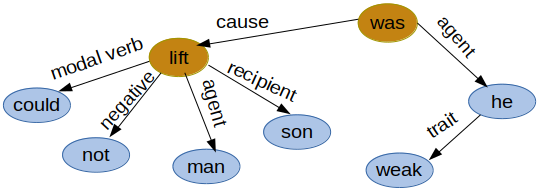
\includegraphics[scale=0.4]{graph_1.png}  
\onslide<2->	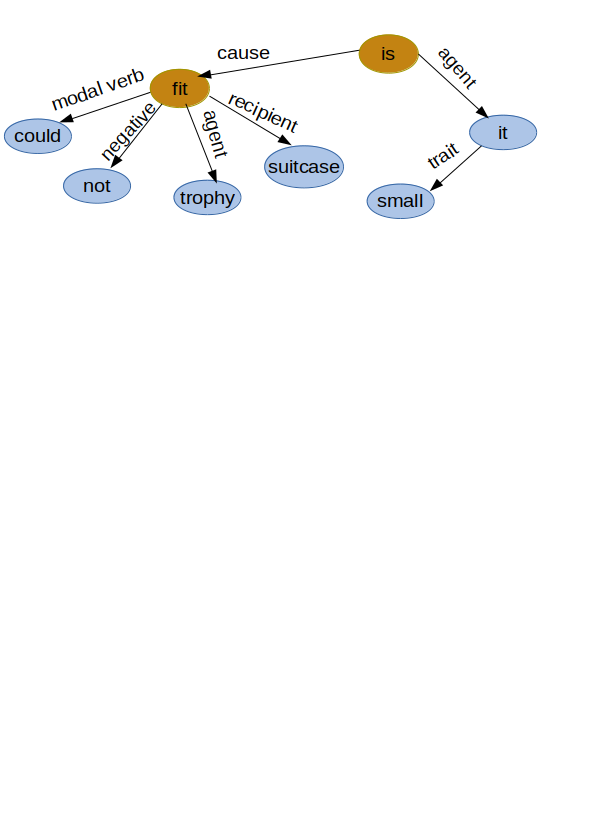
\includegraphics[scale=0.4]{graph_2.png} 
\end{frame}


\begin{frame}{Reasoning}
\onslide<1->	\begin{itemize}
		\item Knowledge required for both examples is about \alert{physical features} 
		\item Similar reasoning rules for categorizing the traits
		\begin{enumerate}
			\normalsize
			\item weak(X) :- lift(X,Y), not lift(modifier, could).
			\item small(Y) :- fit(X,Y), not fit(modifier, could).
		\end{enumerate}
\onslide<2->		\item Reasoning Algorithm
\onslide<2->		\item Change of background knowledge
\onslide<2->		\begin{itemize}
			\normalsize
			\item has\_k(weak,prevents,lift).
		\end{itemize} 
		
	\end{itemize}
\end{frame} 

  
\section{Conclusion}
 
\begin{frame}{Contributions}
    \begin{itemize}
      \normalsize
      \item Overview of different approaches towards WSC
      \item None achieves close to ~90\% accuracy 
      \item We \alert{analyzed} the entire WSC corpus and identified 6 categories
      \item We identified a mistake in the Reasoning Algorithm \\and proposed a correction    
    \end{itemize}
  \end{frame}

\begin{frame}{Future Work}
	\begin{itemize}
		\normalsize
		\item Better Reasoning Algorithm
		\item Knowledge Graphs (RDF) representation
		\item Knowledge-injection neural networks
	\end{itemize}

\end{frame}


  \begin{frame}[standout]
    Thank you!
  \end{frame}

%\begin{frame}{References}
	% This prints the bibliography on the slide
%	\printbibliography
%\end{frame}

\end{document}